\documentclass[11pt]{exam}

\usepackage{amsmath}
\usepackage{graphicx}
\usepackage{geometry}
\usepackage{etoolbox}
\BeforeBeginEnvironment{choices}{\par\nopagebreak\minipage{\linewidth}}
\AfterEndEnvironment{choices}{\endminipage}
\geometry{
a4paper,
total={185mm,257mm},
left=10mm,
top=25mm,
bottom=10mm
}

\begin{document}
\setlength{\voffset}{-0.5in}
\setlength{\headsep}{5pt}

\fbox{\fbox{\parbox{8cm}{\centering
\vspace{2mm}
Testat - Versuch K - Radioaktivitaet 
\vspace{2mm}
}}}
\hspace{2mm}
\makebox[0.25\textwidth]{Name:\enspace\hrulefill} \hspace{5mm}
\makebox[0.2\textwidth]{Datum:\enspace\hrulefill}
\vspace{4mm}

\begin{questions}

\question Wie lautet die Einheit der physikalischen Größe Aktivität?

\begin{choices}
	\choice Gray (Gy)
	\choice Joule (J)
	\choice Meter (m)
	\choice Zeit (t)
	\choice Becquerel (Bq)
\end{choices}

\vspace{3mm}\question Im unten dargestellten Diagramm ist die gemessene Zählrate eines radioaktiven Präparates in Abhängigkeit von der Zeit dargestellt. Wie groß ist die Halbwertszeit?

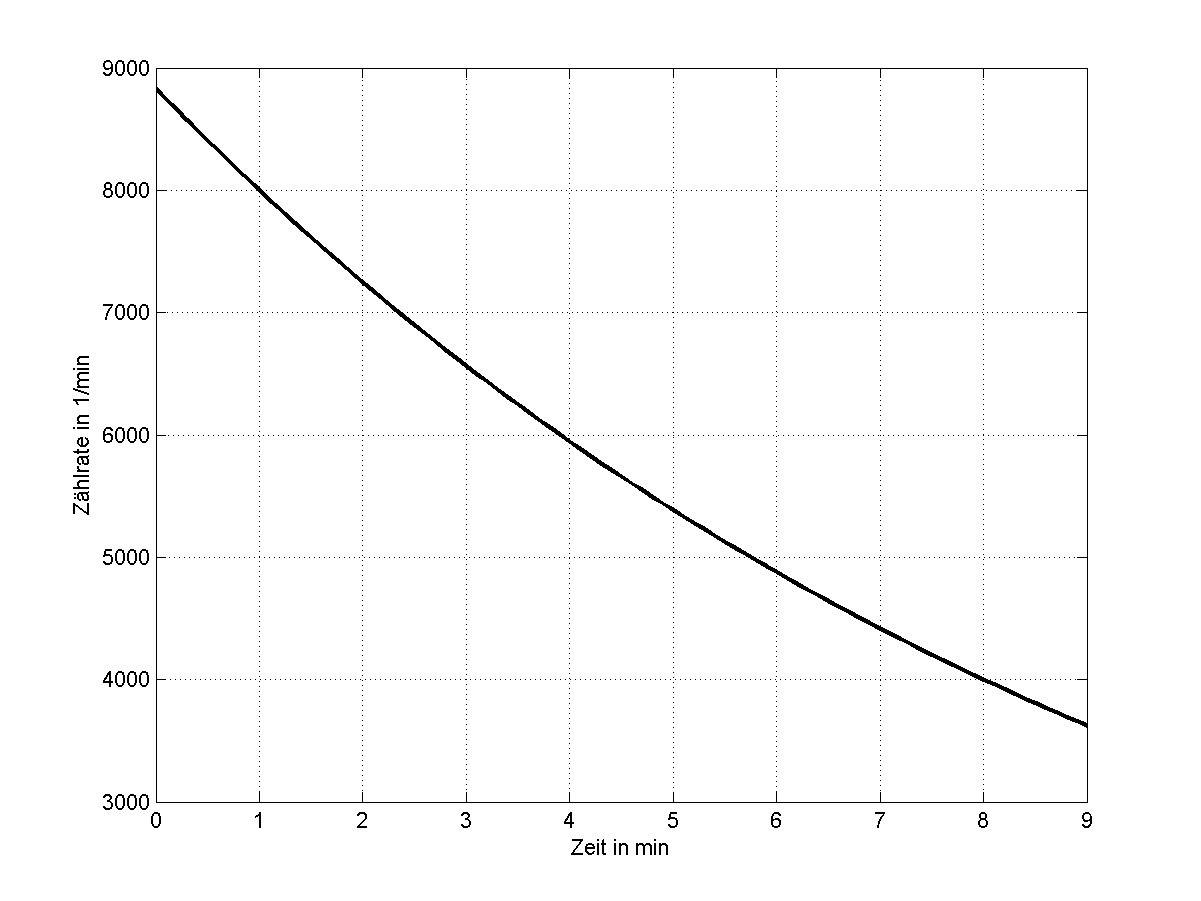
\includegraphics[width=0.4\textwidth]{images/zerfall2.png}

\begin{choices}
	\choice etwa 8 min
	\choice etwa 6 min
	\choice etwa 7 min
	\choice etwa 11 min
	\choice etwa 5 min
\end{choices}

\vspace{3mm}\question Die Halbwertsdicke eines Absorbers beträgt für radioaktives Barium-137m ca. 5 mm. Wieviel Prozent der Strahlung ist nach 12 mm übrig?

\begin{choices}
	\choice 38 %
	\choice 40 %
	\choice 19 %
	\choice 12,5 %
	\choice 25 %
\end{choices}

\vspace{3mm}\question Was hat keinen Einfluss auf die gemessene Zählrate?

\begin{choices}
	\choice Abstand zur Quelle
	\choice Temperatur
	\choice Absorbermaterial
	\choice Aktivität der Quelle
	\choice Absorberdicke
\end{choices}

\vspace{3mm}\question Das Abstandsgesetz beschreibt den Zusammenhang zwischen der Intensität der Strahlung und dem räumlichen Abstand r. Die Intensität ist ...

\begin{choices}
	\choice antiproportional zu r.
	\choice proportional zu r².
	\choice proportional zu r.
	\choice exponentiell von r abhängig.
	\choice proportional zu \( \dfrac{1}{r^2} \).
\end{choices}

\vspace{3mm}\end{questions}

\end{document}
